\documentclass[a4paper,12pt]{insa} % \documentclass[livret]{insa} %- version imprimable recto-verso
\usepackage[utf8]{inputenc}
\usepackage[T1]{fontenc}
\usepackage[french]{babel}
\usepackage{float}
\usepackage{amsmath}

\usepackage{lipsum}          % Pour générer du texte
\usepackage[top=3cm, bottom=3cm, left=3cm, right=3cm]{geometry}

%%%%%%%%%%%%%%%%%%%%%%%%%%%%%%%%%%%%%%%%%%%%%
% OPTIONS                                   %
%%%%%%%%%%%%%%%%%%%%%%%%%%%%%%%%%%%%%%%%%%%%%

\type{Commande optimale}                      % Type du document (par défaut: "Cours")
\titre{Compte rendu du BE \\
suspension (semi) active}   % Titre du documents
\auteur{Ayoub Belafki, Vincent Eychenne}               % Auteur du document
\info{4 AE-SE\\Année 2022-2023}     % Info supplémentaire
%\date{date du jour}                            % Redéfinition de la date (par défaut: "-  Version du {date du jour}  -")
%\setcolorcustom{138,43,226}         %Pour changer la couleur du thème : 
\setcolorinstitutionnel                                    %\setcolorinstitutionnel - \setcolorformation - \setcolorrecherche
                                    %\setcolorinternational - \setcolorentreprise - \setcolorcampus

%%%%%%%%%%%%%%%%%%%%%%%%%%%%%%%%%%%%%%%%%%%%%
% DÉBUT                                     %
%%%%%%%%%%%%%%%%%%%%%%%%%%%%%%%%%%%%%%%%%%%%%
\begin{document}
\dosecttoc{}	  % Sert à générer la table des annexes
\pagestyle{fancy} % Sert à générer les entête et pied de page

\maketitle        % Page de couverture
\makecoverpage    % page de garde
\entete           % entête
\pieddepage       % pied de page

\tableofcontents

\clearpage

\sectionwithoutnumber{Introduction}
Le but de ce bureau d'étude est d'examiner le fonctionnement des suspensions pilotées des voitures, qu'elles soient actives ou semi-actives. Dans un premier temps, nous avons effectué une identification du système en utilisant les principes de la mécanique. Ensuite, nous avons procédé à une analyse du système en boucle ouverte en traçant les courbes pertinentes à l'aide de Matlab. Enfin, nous avons développé une commande optimale en utilisant le critère quadratique, que nous avons ensuite comparé à la méthode du placement des pôles.

\clearpage

\section{Modélisation}
Nous modélisons un système dit de "quart de véhicule", représenté en Figure  \ref{Système "quart de véhicule"}. \\
\begin{center}
    \begin{figure}[H]
        \centering
        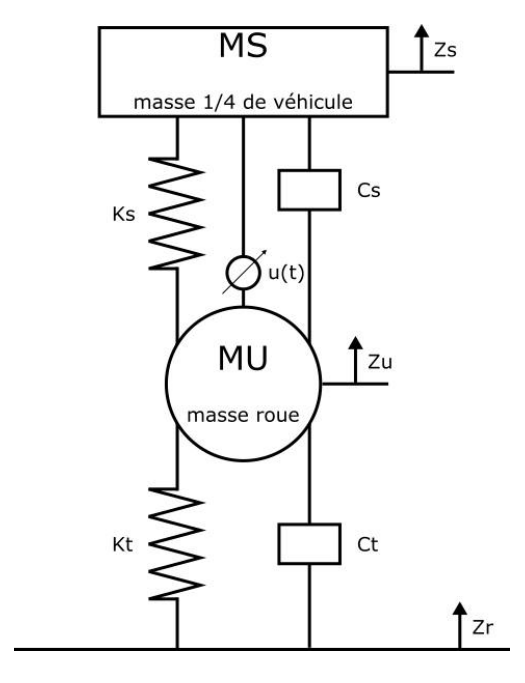
\includegraphics[width=4cm, keepaspectratio]{figures/Quart_vehicule.png}
        \caption{Système "quart de véhicule"}
        \label{Système "quart de véhicule"}
    \end{figure}
\end{center}
Nous avons les variables suivantes : \\
\begin{itemize}
\item[Zs] déplacement vertical de la caisse par rapport à la position d’équilibre
\item[Zu] déplacement vertical de la roue par rapport à la position d’équilibre
\item[Zr] entrée de route (profil de la route)
\item[Ks] raideur du ressort de suspension
\item[Cs] coefficient de frottement de l’amortisseur 
\item[Kt] raideur du pneu
\item[Ct] coefficient d’amortissement du pneu
\end{itemize}

\subsection{Équations du système}
Sur la caisse, les forces suivantes s'appliquent : \\
\begin{itemize}
\item Force du ressort
\item Amortisseur
\item Poids de la caisse
\end{itemize}
Sur la roue, les forces suivantes s'appliquent : \\
\begin{itemize}
\item Force de la raideur du pneu
\item Amortissement du pneu
\item Poids de la roue
\end{itemize}

Nous appliquons ici la deuxième loi de Newton : $\sum \vec{F} = m\times \ddot{a}$\\
Nous considérons les deux déplacements : $Z_u - Z_s$ et $Z_u - Z_r$.\\
Nous obtenons alors : \\
$$
\left \{
\begin{array}{rcl}
M_s\ddot{Z_s} &=& -C_s(\dot{Z_S}-\dot{Z_U}) -K_S(Z_S -Z_U)+u(t) \\
M_U\ddot{Z_U} &=& C_S(\dot{Z_S}-\dot{Z_U})+K_S(Z_S-Z_U)-C_T(\dot{Z_U}-\dot{Z_R})-K_T(Z_U-Z_R) + u(t)
\end{array}
\right.
$$

\subsection{Equation d'état du système}
Nous choisissons : 
\begin{itemize}
\item $X_1 = Z_S - Z_U$ Déplacement relatif caisse/roue,
\item $X_2 = \dot{Z_S}$ Vitesse absolue verticale de la caisse,
\item $X_3 = Z_U - Z_R$ Déplacement relatif roue/sol,
\item $X_4 = \dot{Z_U}$	Vitesse absolue verticale de la roue
\end{itemize}
En injectant les variables d'état dans les équations précédemment obtenues, nous obtenons la représentation d'état suivante : \\
\begin{center}
    \begin{figure}[ht!]
        \centering
        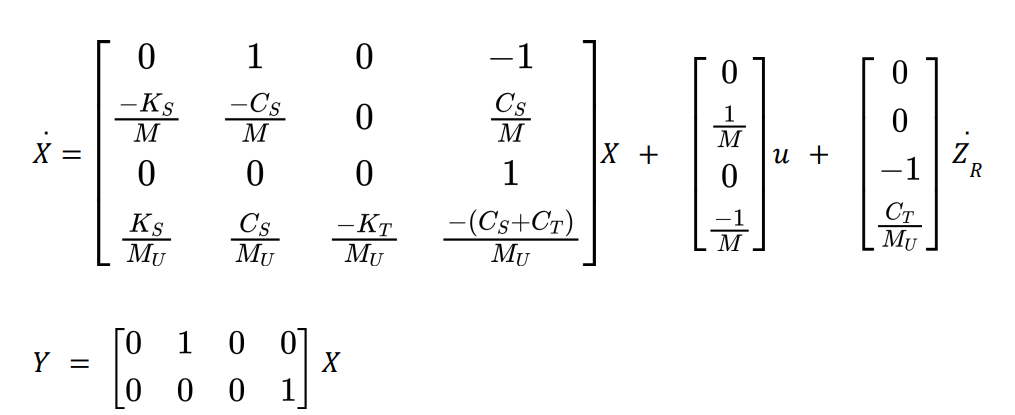
\includegraphics[width=14cm, keepaspectratio]{figures/sys_etat.png}
        \caption{Représentation d'état du système}
        \label{Représentation d'état du système}
    \end{figure}
\end{center}
Nous avons un système de la forme : 
$$
 = 
$$
$$
\left \{
\begin{array}{rcl}
\dot{X} &=& AX + Bu + E\dot{Z_R} \\
Y &=& CX
\end{array}
\right.
$$
\newpage
\section{Analyse en boucle ouverte}
\subsection{Fonctions de transfert}
Nous analysons dans un premier temps le système en boucle ouverte. Cela signifie que l'amortissement est entièrement passif.\\
Nous déterminons, à l'aide de MATLAB, la fonction de transfert de la caisse et de la roue : \\
\begin{center}
    \begin{figure}[H]
        \centering
        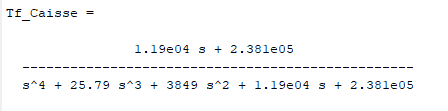
\includegraphics[width=8cm, keepaspectratio]{figures/tf_caisse.png}
    \end{figure}
\end{center}
\begin{center}
    \begin{figure}[H]
        \centering
        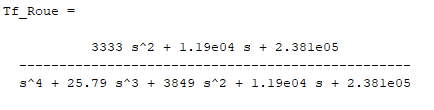
\includegraphics[width=8cm, keepaspectratio]{figures/tf_roue.png}
    \end{figure}
\end{center}
\subsection{Diagrammes de Bode}
Nous obtenons maintenant le diagramme de Bode de la caisse : 
\begin{center}
    \begin{figure}[H]
        \centering
        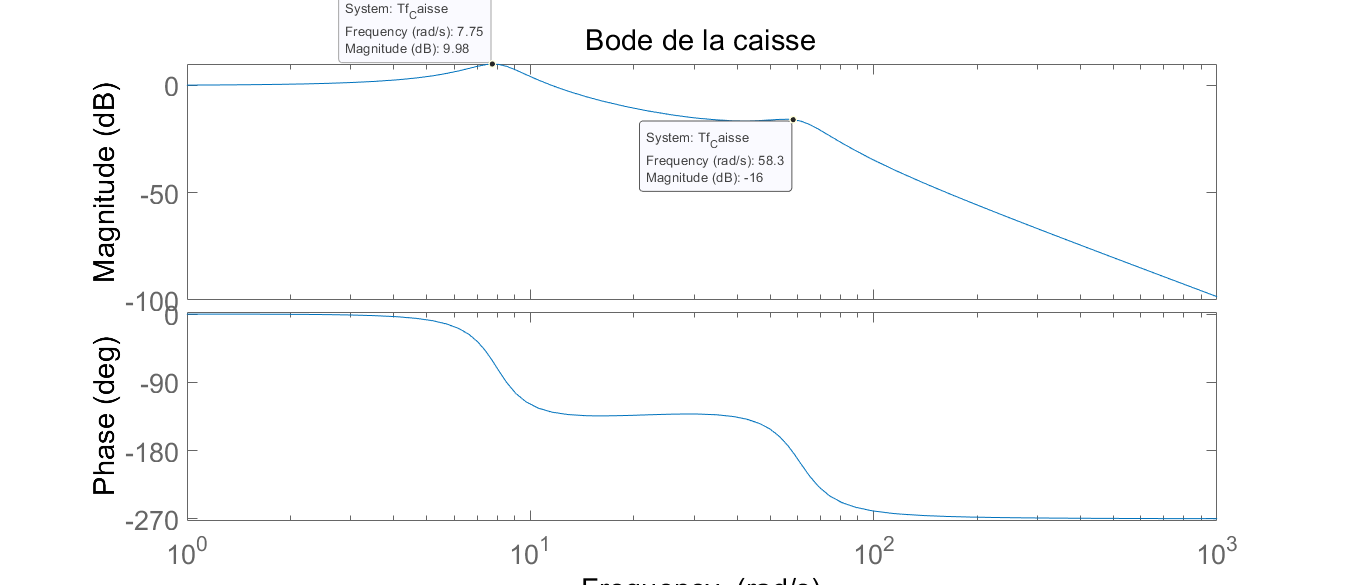
\includegraphics[width=13cm, keepaspectratio]{figures/bode_caisse.png}
        \caption{Bode de la caisse}
        \label{Bode de la caisse}
    \end{figure}
\end{center}
Nous remarquons deux fréquences de résonance : 
\begin{itemize}
\item $\omega_1$ = 7.75 rad/s
\item $\omega_2$ = 58.3 rad/s
\end{itemize}
De même, pour la roue : 
\begin{center}
    \begin{figure}[H]
        \centering
        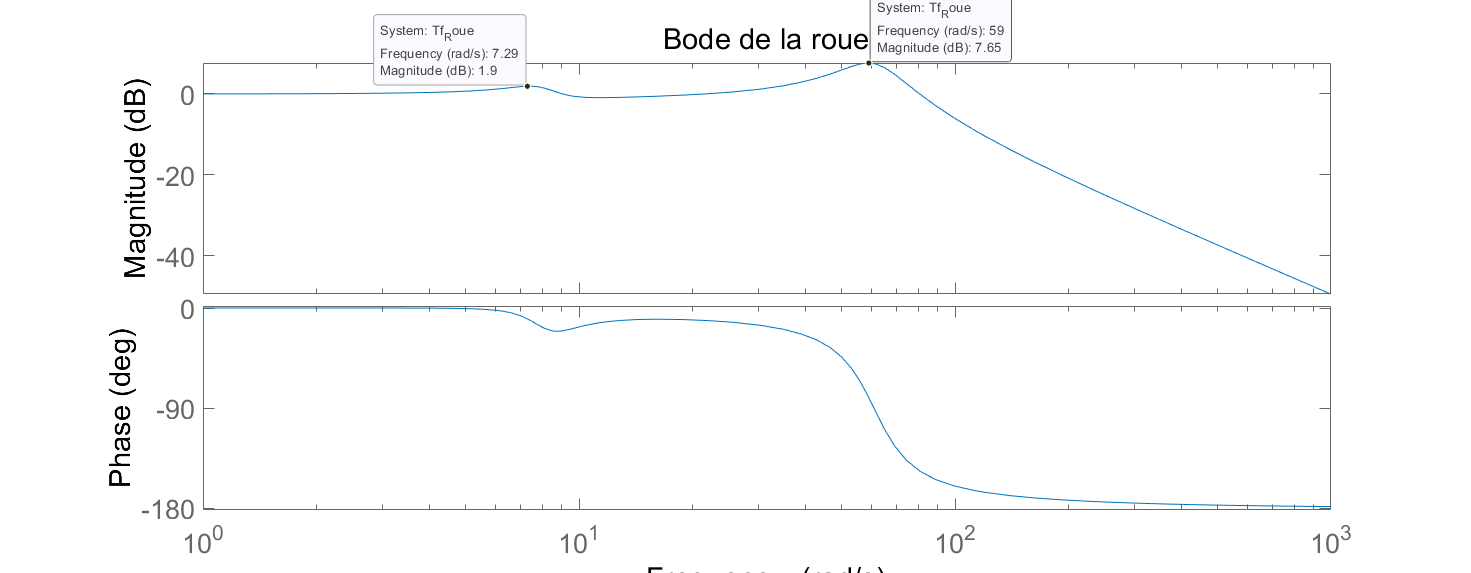
\includegraphics[width=13cm, keepaspectratio]{figures/bode_roue.png}
        \caption{Bode de la roue}
        \label{Bode de la roue}
    \end{figure}
\end{center}

Nous remarquons deux fréquences de résonance : 
\begin{itemize}
\item $\omega_1$ = 7.29 rad/s
\item $\omega_2$ = 59 rad/s
\end{itemize}
\subsection{Réponse à un échelon de 8cm (trottoir)}
Nous regardons maintenant la réponse de notre système à un échelon de 8cm représentant un trottoir.
\begin{center}
    \begin{figure}[H]
        \centering
        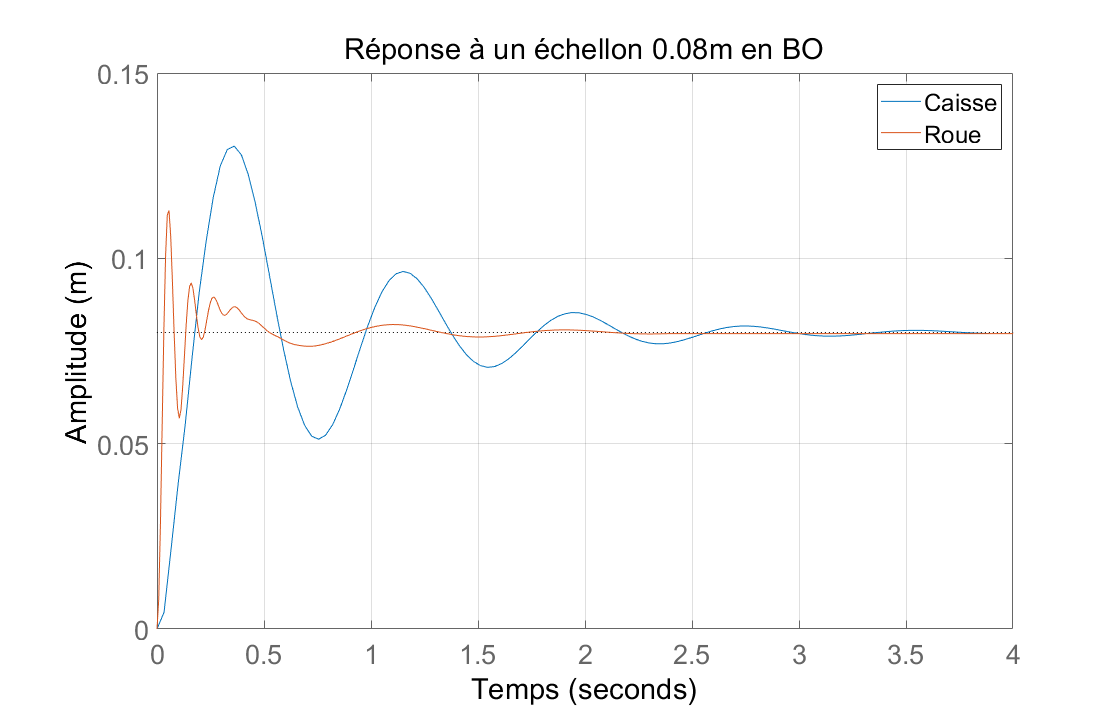
\includegraphics[width=13cm, keepaspectratio]{figures/step_bo.png}
        \caption{Réponse à un échelon en boucle ouverte}
        \label{Réponse à un échelon en boucle ouverte}
    \end{figure}
\end{center}
Nous notons la présence d'oscillations importantes de la caisse (en bleu), réduisant le confort et les performances du véhicule. De plus, la voiture à besoin d'environ 3 secondes avant d'arrêter d'osciller.\\
 Aussi, le comportement de la roue (en orange) est dangereux. La roue décolle du sol lors de l'impact avec le trottoir. Cela nuit à la tenue de route, car le contact avec le sol est rompu.\\
 Afin d'améliorer le comportement, nous devons piloter l'amortisseur.
 \newpage
 \section{Commande optimale}
 \subsection{Coefficients q donnés}
 La commande par retour d'état nous permet de placer un correcteur K minimisant le critère suivant :\\
 $$
 \int_{-\infty }^{+\infty}(X^2_1 q1 + X^2_2 q2 + X^2_3q3+X^2_4 q4 + u^2 r)
 $$
 Avec Q de la forme : 
 $$
 Q = 
 \begin{pmatrix}
 q_1 & 0 & 0 & 0 \\ 
 0 & q_2 & 0 & 0 \\ 
 0 & 0 & q_3 & 0 \\ 
 0 & 0 & 0 & q_4
 \end{pmatrix} 
$$
Afin d'améliorer la performance d'amortissement, nous devons tenir compte des paramètres suivants : 
\begin{itemize}
\item Faible déplacement de la roue, représenté par $X_1$
\item Confort des passagers : vitesse absolue de la roue par rapport à la caisse, représenté par $X_2$
\item Tenue de route : La roue doit rester en contact avec le sol, représenté par $X_3$ 
\end{itemize}
Initialement, nous choisissons les coefficients de Q suivant : 
 $$
 Q = 
 \begin{pmatrix}
 4\times10^8 & 0 & 0 & 0 \\ 
 0 & 10^6 & 0 & 0 \\ 
 0 & 0 & 225\times10^{10} & 0 \\ 
 0 & 0 & 0 & 0
 \end{pmatrix} 
$$
Avec la fonction LQR de MATLAB, nous pouvons déterminer la nouvelle matrice A : \\
$$A_{BF} = A - B \times G$$
Avec G la matrice calculée grâce à la fonction LQR.\\
Nous obtenons alors la réponse à un échelon suivant : \\
\begin{center}
    \begin{figure}[H]
        \centering
        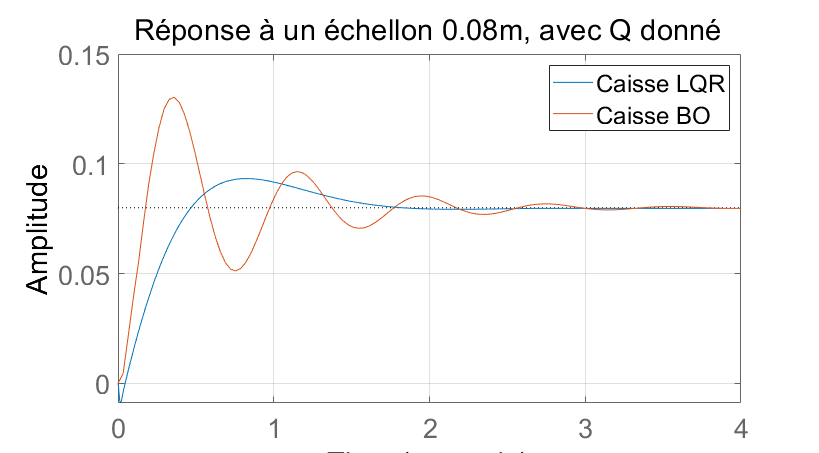
\includegraphics[width=13cm, keepaspectratio]{figures/step_baseLQR.png}
        \caption{Comparaison LQR et BO pour un échelon 8cm}
    \end{figure}
\end{center}
Les mouvements de la caisse sont meilleurs, car sans oscillations. 
Aussi, nous obtenons le diagramme de Bode suivant : 
\begin{center}
    \begin{figure}[H]
        \centering
        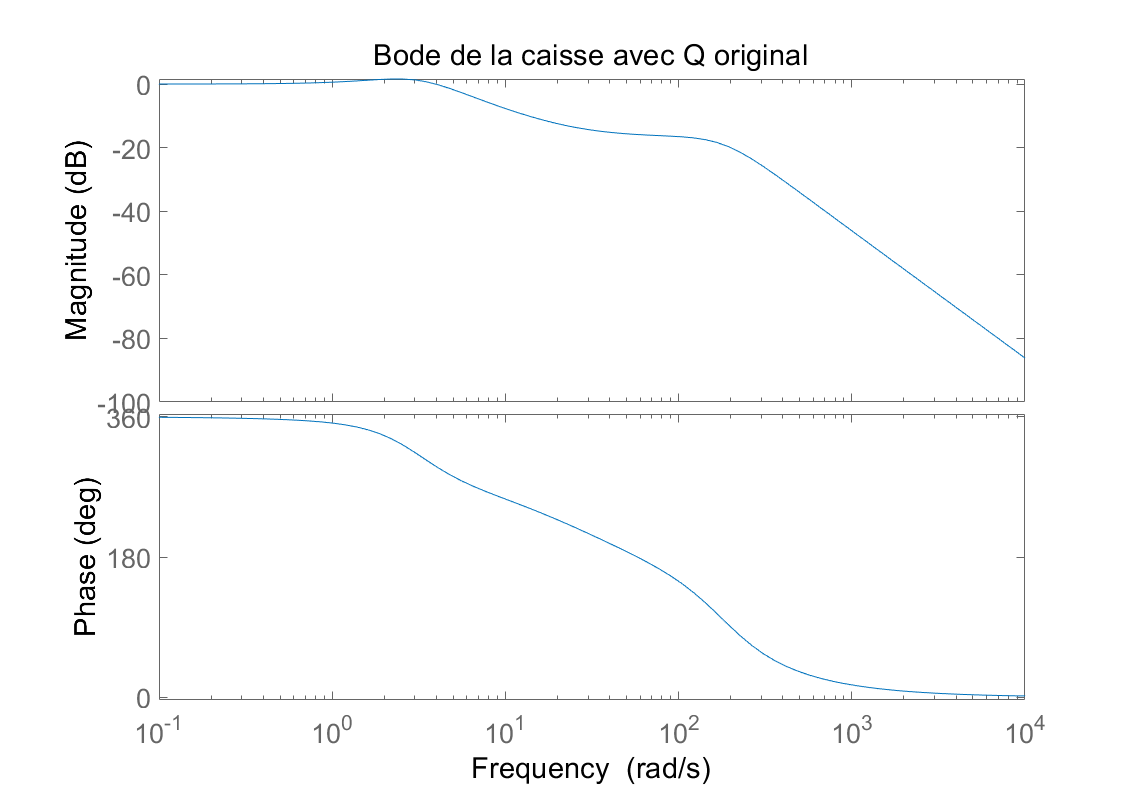
\includegraphics[width=13cm, keepaspectratio]{figures/bode_Q.png}
        \caption{Diagramme de Bode pour Q original}
    \end{figure}
\end{center}
Les résonances ont étés éliminées .\\
Enfin, nous obtenons l'effort de commande suivant : 
\begin{center}
    \begin{figure}[H]
        \centering
        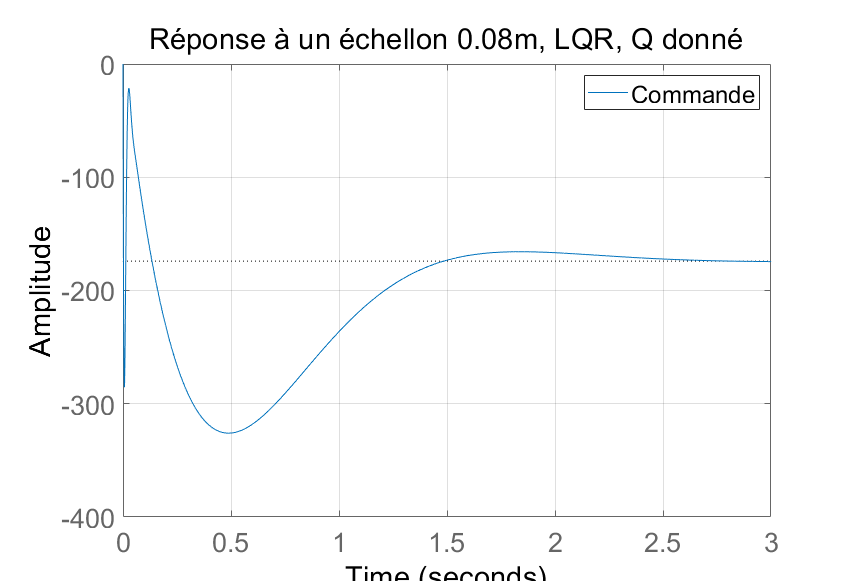
\includegraphics[width=8cm, keepaspectratio]{figures/effort_cmd.png}
        \caption{Diagramme de Bode pour Q original}
    \end{figure}
\end{center}

\subsection{Modification des coefficients}\label{modcoef}
Nous obtenons un résultat optimal pour les coefficients suivants : 
$$
 Q = 
 \begin{pmatrix}
 40\times10^8 & 0 & 0 & 0 \\ 
 0 & 120\times10^6 & 0 & 0 \\ 
 0 & 0 & 0.7\times225\times10^{10} & 0 \\ 
 0 & 0 & 0 & 0
 \end{pmatrix}
$$
La réponse obtenue pour la caisse est la suivante : 
\begin{center}
    \begin{figure}[H]
        \centering
        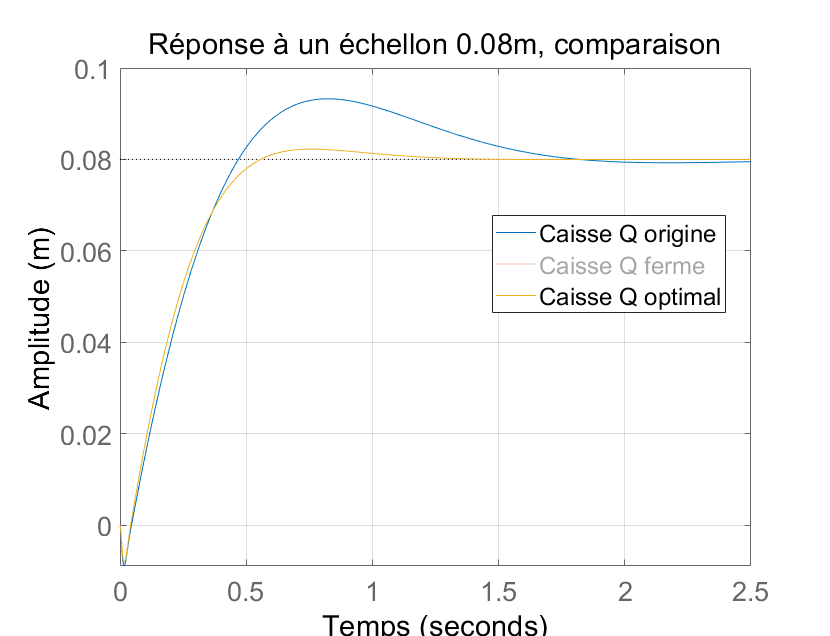
\includegraphics[width=10cm, keepaspectratio]{figures/final_LQR_caisse.png}
        \caption{Réponse de la caisse à un échelon, Q optimal}
    \end{figure}
\end{center}
Le dépassement est maintenant quasi-nul.
La réponse obtenue pour la roue est satisfaisante, même si elle n'a été que légèrement améliorée avec les nouveaux coefficients.\\
\begin{center}
    \begin{figure}[H]
        \centering
        \includegraphics[width=10cm, keepaspectratio]{figures/final_LQR_Roue.png}
        \caption{Réponse de la caisse à un échelon, Q optimal}
    \end{figure}
\end{center}
La commande LQR nous aura permis de grandement améliorer le fonctionnement de notre véhicule, en annulant les oscilliations et en réduisant le dépassement et le temps de réponse.\\
Nous allons maintenant comparer cette méthode avec la méthode par placement de pôles.

\section{Placement de pôles}
 
 Nous récupérons les pôles de la fonction de transfert de la caisse. Nous obtenons les pôles suivants en BO : \\
 Nous avons les pôles suivants : \\
 \begin{center}
    \begin{figure}[H]
        \centering
        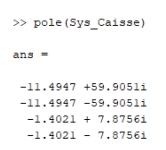
\includegraphics[width=4cm, keepaspectratio]{figures/poles_orig.png}
    \end{figure}
\end{center}
Nous utilisons la fonction place de MATLAB pour calculer $K_p$. Nous choisissons de garder les pôles les plus rapides et imposons deux pôles lents. Nos pôles idéaux sont les suivants : 
 \begin{center}
    \begin{figure}[H]
        \centering
        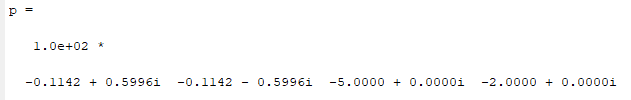
\includegraphics[width=12cm, keepaspectratio]{figures/poles.png}
    \end{figure}
\end{center}
Nous obtenons les gains $K_p$ suivants : \\
 \begin{center}
    \begin{figure}[H]
        \centering
        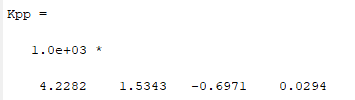
\includegraphics[width=8cm, keepaspectratio]{figures/kpp.png}
    \end{figure}
\end{center}
Notre nouvelle matrice A en boucle fermée devient : 
$$A_p = A-B \times K_p$$
Avec $K_p$ la matrice de gain pour le retour d'état avec le placement de pôles.
Enfin, nous obtenons la réponse suivante, comparée au système en boucle ouverte : \\
 \begin{center}
    \begin{figure}[H]
        \centering
        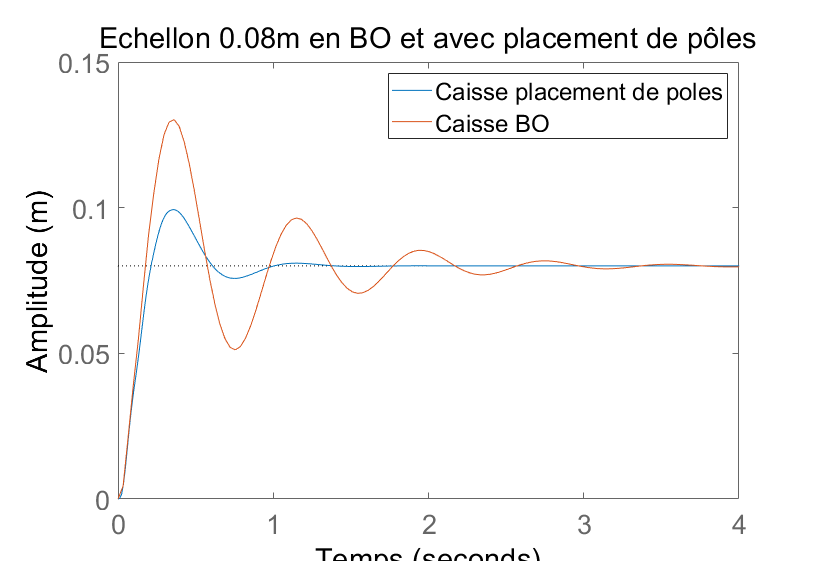
\includegraphics[width=8cm, keepaspectratio]{figures/pp.png}
    \end{figure}
\end{center}

Nous aurions pu ajuster les pôles désirés plus précisément afin d'obtenir une meilleure réponse. Celle obtenue reste néanmoins convaincante.


\section{Conclusion}
Ce bureau d'étude nous aura permis de nous familiariser avec la commande LQR. Nous avons comparé le système en boucle ouverte avec un retour par placement de pôles et une commande LQR. Nous avons pu dans chacun des cas obtenir une bien meilleure réponse qu'en boucle ouverte.\\
Nous avons néanmoins trouvé la commande LQR bien plus simple à implémenter.  
%%%%%%%%%%%%%%%%%%%%%%%%%%%%%%%%%%%%%%%%%%%%%
% ANNEXE                                    %
%%%%%%%%%%%%%%%%%%%%%%%%%%%%%%%%%%%%%%%%%%%%%




%%%%%%%%%%%%%%%%%%%%%%%%%%%%%%%%%%%%%%%%%%%%%
% FIN                                       %
%%%%%%%%%%%%%%%%%%%%%%%%%%%%%%%%%%%%%%%%%%%%%

\makefourthcover    % Quatrième de couverture
\end{document}
